\chapter{Slučajevi upotrebe}\label{ch:slucajevi_upotrebe}

%%%%%%%%%%%%%%%%%%%%%%
\section{Prijava korisnika uz pomoć GitHub IdP}

\textbf{Kratak opis}: Korisnik se prijavljuje sa sopstvenim kredencijalima

\textbf{Učesnici}: Korisnik, Veb aplikacija, Gateway, GitHub Identity Provider (IdP)

\textbf{Postuslov}: Korisnik je prijavljen

\textbf{Glavni tok}:
\begin{enumerate}
    \item Korisnik klikne na dugme za prijavu
    \item Sistem šalje zahtev prema Gateway-u za prijavu
    \item Gateway vraća preusmeravanje (302 Redirect) na stranicu za prijavu 
    provajdera identiteta (u ovom slučaju GitHub)
    \item Šalje se zahtev za dobijanje stranice za prijavu provajdera 
    identiteta
    \item GitHub šalje stranicu za prijavu korisnika
    \item Korisnik unosi svoje kredencijale
    \item Korisnik šalje zahtev za prijavu klikom na dugme
    \item GitHub dobija podatke za prijavu i nakon uspešnog prijavljivanja 
    šalje kod za pristup veb aplikaciji
    \item Veb aplikacija prosleđuje Gateway-u kod za pristup
    \item Gateway, uz zahtev za dobijanje podataka o korisniku, prosleđuje 
    kod za pristup GitHub-u 
    \item GitHub Gateway-u vraća podatke o korisniku
    \item Na osnovu dobijenih podataka Gateway generiše JWT token
    \item Gateway šalje JWT token Veb aplikaciji
    \item Veb aplikacija omogućava prikaz zaštićene stranice korisniku 
    i čuva JWT token za buduće komunikacije
\end{enumerate}

\begin{figure}[H]
    \centering
    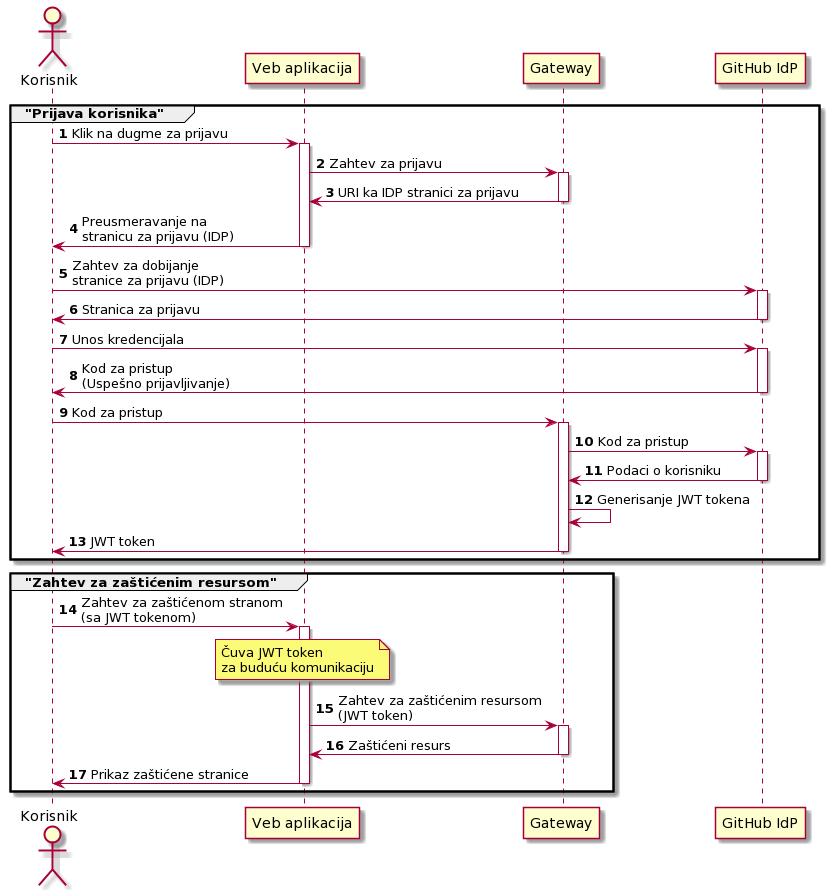
\includegraphics[width=0.75\textwidth]{prijava_korisnika}
    \caption{Dijagram sekvence -- prijava korisnika}
\end{figure}


%%%%%%%%%%%%%%%%%%%%%%
\section{Kreiranje projekta}

\textbf{Kratak opis}: Korisnik ima mogućnost da kreira novi projekat

\textbf{Učesnici}: Korisnik

\textbf{Postuslov}: Projekat je kreiran

\textbf{Glavni tok}:
\begin{enumerate}
    \item Sistem prikazuje opciju za kreiranje novog projekta
    \item Korisnik bira akciju za kreiranje novog projekta
    \item Sistem prikazuje formu sa tekstualnim poljima za unos podataka o projektu
    \item Korisnik unosi naziv projekta, vlasnika Github repozitorijuma, 
    GitHub repozitorijum i putanju na kojoj će se čuvati podaci o projektu
    \item Korisnik klikne na dugme za kreiranje projekta
    \item Sistem čuva projekat
    \item Sistem korisniku vraća stranicu sa podacima o projektu
\end{enumerate}

\begin{figure}[H]
    \centering
    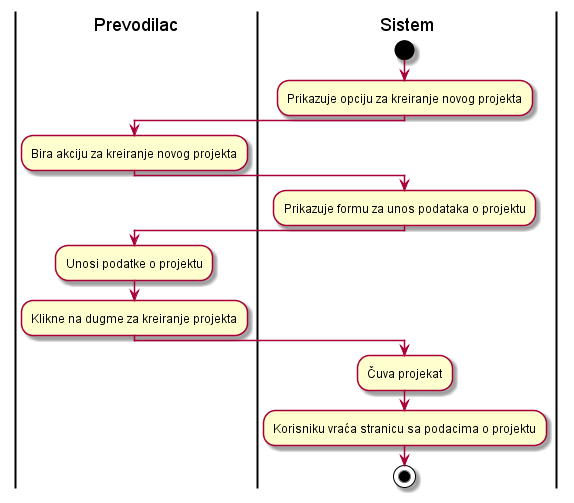
\includegraphics[width=0.75\textwidth]{kreiranje_projekta}
    \caption{Dijagram aktivnosti - kreiranje projekta}
\end{figure}


%%%%%%%%%%%%%%%%%%%%%%
\section{Uvoz prevoda}

\textbf{Kratak opis}: Korisnik želi da uveze prevode sa GitHub-a

\textbf{Učesnici}: Korisnik

\textbf{Postuslov}: Korisnik se nalazi na projektu u koji želi da uveze prevode

\textbf{Glavni tok}:
\begin{enumerate}
    \item Sistem prikazuje opcije za uvoz i izvoz projekta
    \item Korisnik bira akciju za izvoz projekta
    \item Sistem prikazuje modal sa porukom da će se uvozom projekta sve 
    izmene koje nisu izvezene izgubiti
    \item Korisnik unosi naziv projekta, vlasnika Github repozitorijuma, 
    GitHub repozitorijum i putanju na kojoj će se čuvati podaci o projektu
    \item Korisnik klikne
    \begin{enumerate}
        \item na dugme OK ukoliko nema prevoda koji nisu izvezeni
        \begin{enumerate}
            \item Sistem uvozi projekat
            \item Sistem zatvara modal
        \end{enumerate}        
        \item na dugme Cancel kako bi obustavio uvoz
        \begin{enumerate}
            \item Sistem zatvara modal
        \end{enumerate}
    \end{enumerate}        
    
\end{enumerate}

\begin{figure}[H]
    \centering
    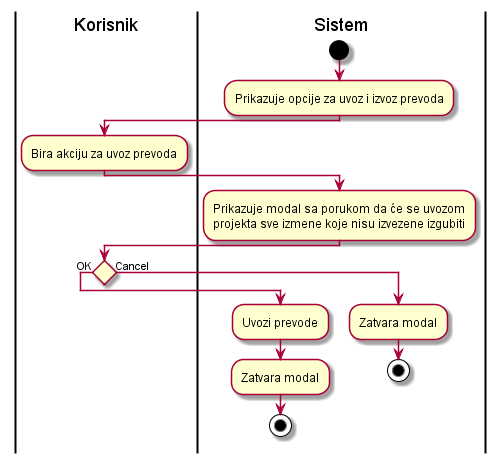
\includegraphics[width=0.75\textwidth]{uvoz_prevoda}
    \caption{Dijagram aktivnosti -- uvoz prevoda}
\end{figure}


%%%%%%%%%%%%%%%%%%%%%%
\section{Izmena prevoda}

\textbf{Kratak opis}: Korisnik vrši izmene kako bi dodao novi prevod ili izmenio postojeći

\textbf{Učesnici}: Korisnik

\textbf{Postuslov}: Uspešno izvršena izmena prevoda

\textbf{Glavni tok}:
\begin{enumerate}
    \item Sistem prikazuje listu prevoda sa odgovarajućim ključevima
    \item Korisnik klikne na željeni ključ za koji želi da unese ili izmeni prevod
    \item Sistem vraća tekstualna polja za unos za onoliko jezika koliko je u tom 
    trenutku dostupno za izabrani ključ
    \item Korisnik unosi ili menja jedan ili više prevoda
    \item Prevod se automatski šalje na čuvanje u trenutku kada tekstualno polje izgubi fokus
    \item Sistem čuva izmenjeni prevod
\end{enumerate}

\begin{figure}[H]
    \centering
    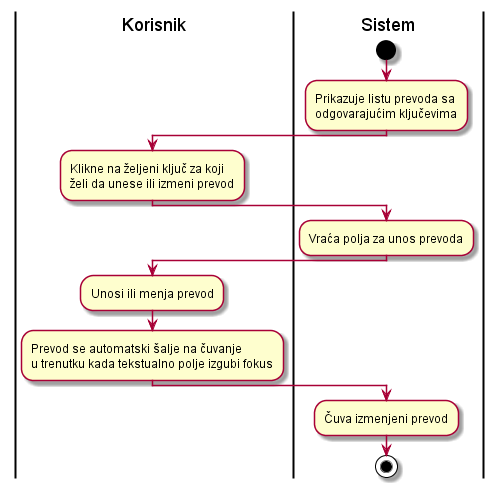
\includegraphics[width=0.75\textwidth]{izmena_prevoda}
    \caption{Dijagram aktivnosti -- izmena prevoda}
\end{figure}


%%%%%%%%%%%%%%%%%%%%%%
\section{Izvoz prevoda}

\textbf{Kratak opis}: Korisnik želi da izveze prevode izabranog projekta i 
na taj način kreira pull request na GitHub-u

\textbf{Učesnici}: Korisnik

\textbf{Preduslov}: Korisnik se nalazi na projektu koji želi da izveze

\textbf{Postuslov}: Uspešno izvezen sadrđaj projekta

\textbf{Glavni tok}:
\begin{enumerate}
    \item Sistem prikazuje opcije za uvoz i izvoz prevoda
    \item Korisnik bira akciju za izvoz prevoda
    \item Sistem prikazuje modal sa formom za unos naslova i opisa 
    zahteva za promenu (eng. Pull Request)
    \item Korisnik unosi naslov i opis u tekstualna polja
    \item Korisnik klikne na dugme OK
    \item Sistem pokreće akciju izvoza projekta
    \item Na GitHub-u se kreira zahtev za promenu sa izmenjenim fajlovima za prevode
\end{enumerate}

\begin{figure}[H]
    \centering
    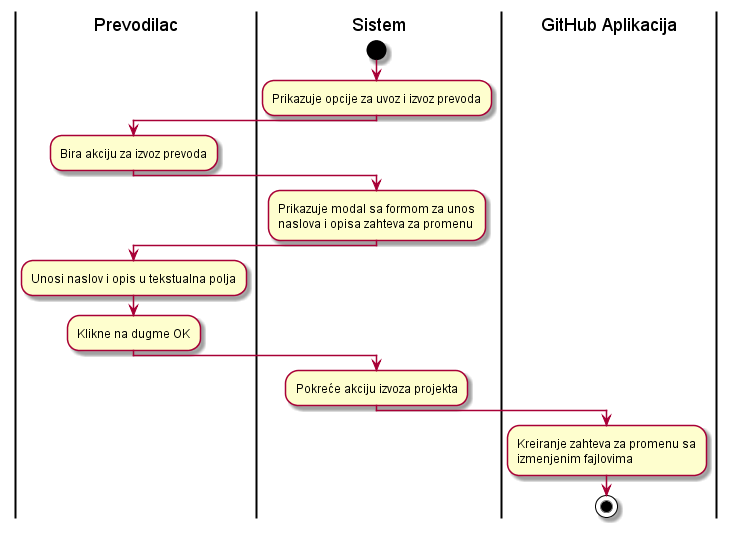
\includegraphics[width=0.75\textwidth]{izvoz_prevoda}
    \caption{Dijagram aktivnosti -- izvoz prevoda}
\end{figure}
